% DAQCNN pipeline schematic, v2.
% Monochrome style matching the QGARS paper figure: black outlines, white/gray
% fills, Computer Modern labels, dashed group boxes with (a)/(b)/... tags,
% solid thin arrows for data flow, dashed arrows for the loss/gradient path.
% Compile: pdflatex daqcnn_pipeline_v2.tex
\documentclass[tikz,border=8pt]{standalone}
\usepackage{amsmath,amssymb,bm}
\usetikzlibrary{positioning, arrows.meta, calc, fit}

% Rydberg atom: small circle with radiating arcs above and below
\tikzset{
  pics/atom/.style={code={
    \draw[line width=0.5pt] (0,0) circle (0.075);
    \foreach \r in {0.14,0.20,0.26}{
      \draw[line width=0.35pt] (55:\r) arc (55:125:\r);
      \draw[line width=0.35pt] (-125:\r) arc (-125:-55:\r);
    }
  }}
}

% 3x3 patch grid (0.9 x 0.9), shaded cells; #1 = seed offset for the grays
\newcommand{\patchgrid}[3]{% x, y, seed
  \begin{scope}[shift={(#1,#2)}]
    \foreach \i in {0,1,2}{
      \foreach \j in {0,1,2}{
        \pgfmathtruncatemacro{\gg}{mod(#3+\i*23+\j*31+\i*\j*7,55)+8}
        \fill[gray!\gg] (\i*0.3,\j*0.3) rectangle +(0.3,0.3);
      }
    }
    \draw[step=0.3, line width=0.4pt] (0,0) grid (0.9,0.9);
  \end{scope}
}

\begin{document}
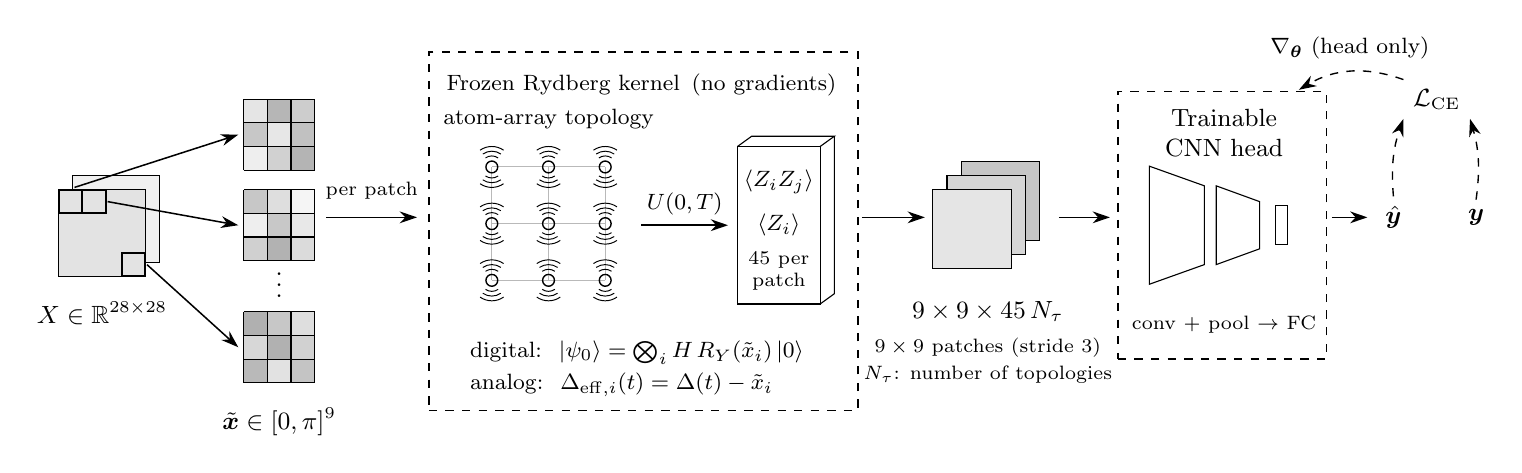
\begin{tikzpicture}[
    >={Stealth[length=2.2mm,width=1.5mm]},
    font=\small,
    arr/.style={->, line width=0.55pt},
    larr/.style={->, dashed, line width=0.5pt},
    gbox/.style={draw, dashed, line width=0.5pt, inner sep=0pt},
    lbl/.style={font=\normalsize}
  ]

% =================== (a) input image + patch extraction ===================
% stacked input images (light gray)
\fill[gray!12] (0.18,-0.62) rectangle +(1.1,1.1);
\draw (0.18,-0.62) rectangle +(1.1,1.1);
\fill[gray!22] (0,-0.8) rectangle +(1.1,1.1);
\draw (0,-0.8) rectangle +(1.1,1.1);
% three distinct 3x3 patch regions on the front image (stride-like tiling)
% stride-3 tiling: first two patches flush in the top-left corner,
% adjacent to each other; last patch flush in the bottom-right corner
\draw[line width=0.7pt] (0,0) rectangle +(0.3,0.3);
\draw[line width=0.7pt] (0.3,0) rectangle +(0.3,0.3);
\draw[line width=0.7pt] (0.8,-0.8) rectangle +(0.3,0.3);
\node[anchor=north, align=center] at (0.55,-1.0)
  {$X\in\mathbb{R}^{28\times 28}$};

% column of extracted patches: patch, patch, vdots, patch
\patchgrid{2.35}{0.55}{5}
\patchgrid{2.35}{-0.6}{29}
\node at (2.8,-0.81) {$\vdots$};
\patchgrid{2.35}{-2.15}{47}
\node[anchor=north, align=center] at (2.8,-2.35)
  {$\tilde{\bm{x}}\in[0,\pi]^9$};

% patch-extraction arrows: one from each marked region to its patch
\draw[arr] (0.2,0.33) -- (2.28,1.0);
\draw[arr] (0.62,0.15) -- (2.28,-0.15);
\draw[arr] (1.12,-0.65) -- (2.28,-1.7);

% flow into quantum box
\draw[arr] (3.4,-0.05) -- node[above=3pt, font=\scriptsize, pos=0.5]{per patch} (4.55,-0.05);

% =================== (b) frozen quantum kernel ===================
% dashed group box first (drawn behind contents)
\node[gbox, fit={(4.7,-2.5) (10.15,2.05)}] (qbox) {};
\node[anchor=north, font=\footnotesize] at (7.4,1.9) {Frozen Rydberg kernel\enspace(no gradients)};

% atom array (3x3 with neighbor bonds)
\begin{scope}[shift={(5.5,-0.85)}]
  \foreach \i in {0,1,2}{
    \draw[gray!55, line width=0.35pt] (0,\i*0.72) -- (1.44,\i*0.72);
    \draw[gray!55, line width=0.35pt] (\i*0.72,0) -- (\i*0.72,1.44);
  }
  \foreach \i in {0,1,2}{
    \foreach \j in {0,1,2}{
      \pic at (\i*0.72,\j*0.72) {atom};
    }
  }
\end{scope}
\node[anchor=south, align=center, font=\footnotesize] at (6.22,0.95)
  {atom-array topology};

% encoding formulas inside the box, under atoms + slab
\node[anchor=north west, align=left, font=\footnotesize] at (5.1,-1.5) {%
  digital:\; $|\psi_0\rangle=\bigotimes_i H\,R_Y(\tilde{x}_i)\,|0\rangle$\\[2pt]
  analog:\; $\Delta_{\mathrm{eff},i}(t)=\Delta(t)-\tilde{x}_i$};

% evolution arrow to measurement slab
\draw[arr] (7.4,-0.15) -- node[above, font=\footnotesize]{$U(0,T)$} (8.5,-0.15);

% measurement slab (complete 3D box: front face + top + right side)
\begin{scope}[shift={(8.62,-1.15)}]
  \draw (0,0) rectangle (1.05,2.0);                          % front face
  \draw (0,2.0) -- (0.18,2.13) -- (1.23,2.13) -- (1.05,2.0); % top face
  \draw (1.23,2.13) -- (1.23,0.13) -- (1.05,0);              % right face
  \node[font=\footnotesize] at (0.525,1.55) {$\langle Z_i Z_j\rangle$};
  \node[font=\footnotesize] at (0.525,1.0) {$\langle Z_i\rangle$};
  \node[font=\scriptsize, align=center] at (0.525,0.42) {45 per\\patch};
\end{scope}

% flow to feature map
\draw[arr] (10.2,-0.05) -- (11.0,-0.05);

% =================== (c) quantum feature map ===================
\fill[gray!45] (11.46,-0.34) rectangle +(1.0,1.0);
\draw (11.46,-0.34) rectangle +(1.0,1.0);
\fill[gray!32] (11.28,-0.52) rectangle +(1.0,1.0);
\draw (11.28,-0.52) rectangle +(1.0,1.0);
\fill[gray!20] (11.1,-0.7) rectangle +(1.0,1.0);
\draw (11.1,-0.7) rectangle +(1.0,1.0);
\node[anchor=north, align=center] at (11.8,-1.0)
  {$9\times 9\times 45\,N_{\tau}$\\[1pt]
   {\scriptsize $9\times 9$ patches (stride $3$)}\\[-1pt]
   {\scriptsize $N_{\tau}$: number of topologies}};

% flow to head
\draw[arr] (12.7,-0.05) -- (13.35,-0.05);

% =================== (d) trainable CNN head ===================
% dashed group box (drawn first), title inside its top edge
\node[gbox, fit={(13.45,-1.85) (16.1,1.55)}] (hbox) {};
\node[anchor=north, align=center] at (14.8,1.45) {Trainable\\CNN head};

% conv trapezoids, narrowing
\draw (13.85,-0.9) -- (14.55,-0.65) -- (14.55,0.35) -- (13.85,0.6) -- cycle;
\draw (14.7,-0.65) -- (15.25,-0.45) -- (15.25,0.15) -- (14.7,0.35) -- cycle;
% FC bar
\draw (15.45,-0.4) rectangle +(0.16,0.5);
\node[anchor=north, align=center, font=\scriptsize] at (14.8,-1.18)
  {conv $+$ pool $\to$ FC};

% output
\draw[arr] (16.17,-0.05) -- (16.62,-0.05);
\node (yhat) at (16.95,-0.05) {$\hat{\bm{y}}$};
\node (ytrue) at (18.0,-0.05) {$\bm{y}$};

% =================== loss + gradient path (dashed) ===================
\node (loss) at (17.5,1.45) {$\mathcal{L}_{\mathrm{CE}}$};
\draw[larr] (yhat.north) to[bend left=12] (loss.south west);
\draw[larr] (ytrue.north) to[bend right=12] (loss.south east);
% gradient flows back into the head only (enter at top-right corner, label above)
\draw[larr] (loss.north west) to[bend right=25]
  node[above, font=\footnotesize, pos=0.5, yshift=1pt]{$\nabla_{\bm{\theta}}$ (head only)}
  (15.75,1.57);

\end{tikzpicture}
\end{document}
